\documentclass[10pt,letterpaper,spanish,twoside]{report}

\usepackage{practica}
\usepackage{graphicx}
\usepackage{float}
\DeclareGraphicsExtensions{.bmp,.png,.pdf,.jpg}
\newcommand{\docdate}{
  \vspace{2em}
   \begin{flushright}
     Ciudad de México. \datedayname~\today.
   \end{flushright}
  \vspace{2em}
}

\begin{document}
\docdate

\begin{center}
 \textsc{\asignatura}\vspace{.2em}
\end{center}

\textsc{Manual del profesor}

\textsc{Práctica 1. aplicación de filtros analógicos tipo Butterworth pasa bajas a señales biomédicas reales}

\textsc{Objetivo:} Aplicar los conocimientos sobre el diseño de filtros Butterworth pasa bajas para procesamiento de señales biomédicas reales simulando su adquisición en tiempo real

\textsc{Actividades}
\begin{enumerate}
 \item Se descarga el archivo de audio 'BPW$\_$noise.wav' disponible en goo.gl/8TvoDM
 \item Utilzando el osciloscopio se procede a obtener la FFT de la señal de audio. Esto se debe hacer conectando el cable de audio de 3.5 mm al preamplificador previamente diseñado, y conectando la salida de dicho amplificador al osciloscopio.
 \item Se observará la FFT mostrada en la figura%~\ref{Figura de FFT en osciloscopio} 
 \\En dicha imagen podemos observar que el rudio se encuentra entre las frecuencias de 90 y 120 Hz. Si se desea modificar este contenido espectral se recomienda revisar el scrip 'SeñalesUtilizadas' disponible en el repositorio actual.
 \\ INSERTAR IMAGEN DE OSCILOSCOPIO
 \item Se recomienda diseñar un filtro pasa bajas con frecuencia de corte de 70 Hz. Para modificar el diseño del filtro se recomienda el uso del script 'Diseño de filtros' el cuál cuenta con una función creada para obtener los valores de resistencias y capacitores para lograr el filtro deseado. Dicha función se basa en las ecuaciones descritas en el documento 'MT-222' de la marca 'Analog Devices', el cuál consiste en un mini tutorial respecto al diseño de filtros utilizando la topología Sallen-Key.
 \item Ya obtenidos todos los valores de resistencias y capacitores se procede a armar el circuito mostrado en la figura~\ref{contexto:PB2}
 \\Así también, se muestra en la ecuación~\eqref{FT_n2} la función de transferencia del filtro.
 \begin{equation}
 	H(s)=\frac{522.299K}{s^2+622.003s+193.444K}\label{FT_n2}
 \end{equation}  
 \begin{figure}[H]
 	\centering
 	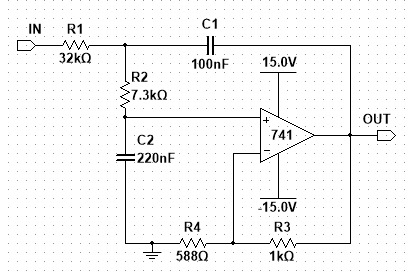
\includegraphics[scale=0.4]{PB2.PNG}
 	\caption{Circuito eléctrico de filtro pasa bajas orden 2}
	\label{contexto:PB2}
 \end{figure}
 \item Se procede a realizar la caracterización del filtro realizando 15 mediciones por década y 10 mediciones al rededor de la frecuencia de corte. Se deben registrar datos de magnitud y fase.
 \\ En la figura \ref{contexto:RF_2} se observa la respuesta en frecuencia del filtro. Es posible observar que la frecuencia de corte se encuentra en alrededor de los 62 Hz.
 \\Los datos obtenidos pueden consultarse en el archivo 'P1$\_$n2$\&$4$\_$caracterizacion.ipynb'.
 \begin{figure}[H]
 	\centering
 	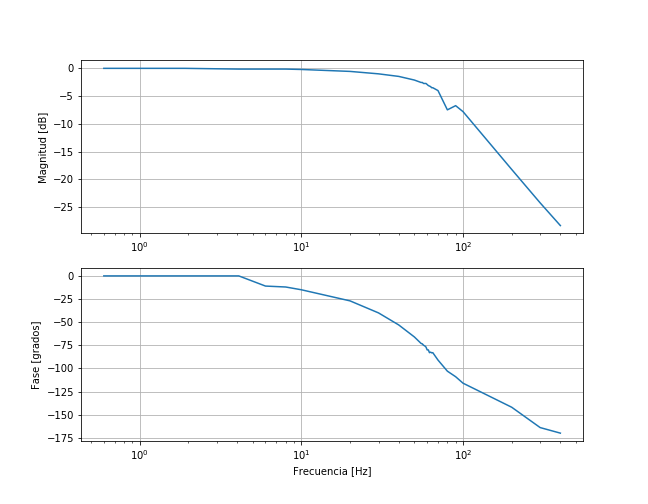
\includegraphics[scale=0.5]{RF_PB2.PNG}
 	\caption{Respuesta en frecuencia de filtro pasa bajas orden 2}
	\label{contexto:RF_2}
 \end{figure}
 \begin{enumerate}
  \item Una ves verificado que se obtuvo al frecuencia de corte deseada o una cercana a ella, se procede a filtrar la señal de audio, recordando ingresarla primeramente al sistema preamplificador.
  \item Se debe realizar una comparación entre la señal original y filtrada y almacenar los datos de dicha comparación. Se recomienda que se obtenga una imagen donde se observe la comparación entre señal original y señal filtrada, así como la FFT de la señal filtrada. En las figuras no y no se muestran la comparción de señales y la FFT de la señal filtrada respectivamente.
  \\ INSERTAR IMAGENES DE OSCILOSCOPIO
 \end{enumerate}
 \item Para el diseño del filtro pasa bajas orden 4 se sugiere utilizar una frecuencia de corte de 75Hz. En este caso, se utiliza de igual forma el script 'Diseño de filtros' pero realizando el diseño del filtro en sus dos etapas que lo componen.
 \item Ya obtenidos los valores de resistencias y capacitores se procede a implementar circuito de la figura \ref{contexto:PB4}
 \\En la ecuación~\eqref{FT_n4} se muestra la función de transferencia del filtro orden 4
 \begin{equation}
 	H(s)=\frac{228.685K}{s^2+360.639s+222.066K} \frac{399.718K}{s^2+870.708s+222.066K}\label{FT_n4}
 \end{equation}
 \begin{figure}[H]
 	\centering
 	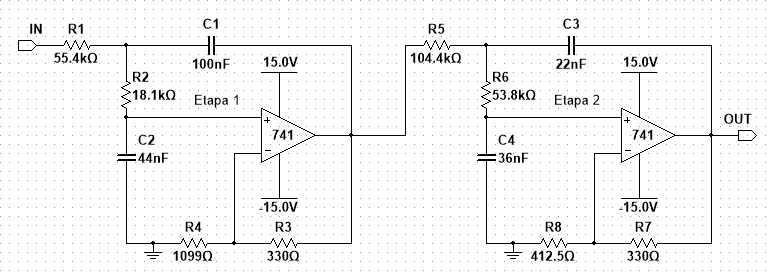
\includegraphics[scale=0.7]{PB4.PNG}
 	\caption{Circuito eléctrico de filtro pasa bajas orden 4}
	\label{contexto:PB4}
 \end{figure}
 \item Posteriormente se procede a realizar la caracterización de dicho filtro tomando en cuenta las consideraciones mencionadas en el punto 6.
 \\ En la figura \ref{contexto:RF_4} se observa la respuesta en frecuencia del filtro pasa bajas orden 4. Es posible observar que la frecuencia de corte se encuentra en alrededor de 80 Hz.
 \\Los datos obtenidos pueden consultarse en el archivo 'P1$\_$n2$\&$4$\_$caracterizacion.ipynb'.
 \begin{figure}[H]
 	\centering
 	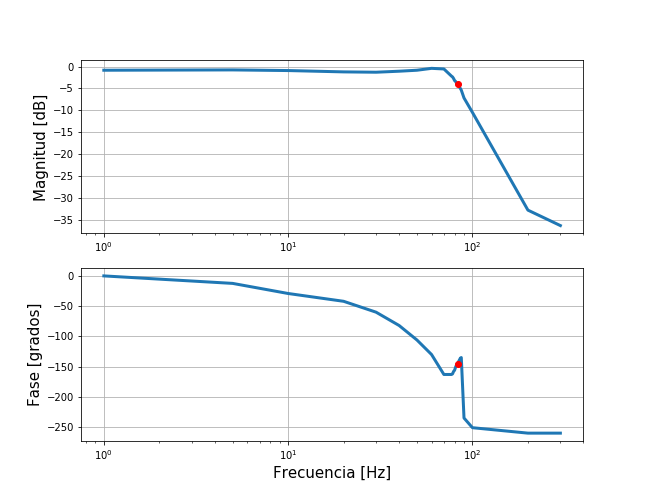
\includegraphics[scale=0.4]{RF_PB4.PNG}
 	\caption{Respuesta en frecuencia de filtro pasa bajas orden 4}
	\label{contexto:RF_4}
 \end{figure}
 \begin{enumerate}
 \item Verificada la frecuencia se procede a realizar el filtrado de la señal y a obtener la comparación de señales y FFT correspondientes. En las figuras no y no se muestra la comparación de señales y la FFT de la señal filtrada respectivamente.
 \\INSERTAR FIGURA DE SEÑAL CONTAMINADA Y FILTRADA EN EL OSCILOSCOPIO
 \end{enumerate}
\end{enumerate}


%\textsc{Nota}
%\vspace{2em}
\vfill
\begin{flushright}
\textsc{Elaboró:\\
Ma. del Rosario Aguilar Cruz\\
Enrique Mena Camilo}
\end{flushright}

\end{document}